\documentclass{article}
\usepackage{graphicx}
\usepackage{paralist} % needed for compact lists
\usepackage[normalem]{ulem} % needed by strike
\usepackage[urlcolor=blue,colorlinks=true]{hyperref}
\usepackage[utf8x]{inputenc}  % char encoding
\usepackage[frenchb]{babel}  % user defined

\title{Langages de balisage légers et logiciels de conversion de documents}
\author{Nicolas Poulain}
\begin{document}
%\maketitle
\clearpage


\section*{Isaac Newton}

\textbf{Sir Isaac Newton} (4 janvier 1643 - 31 mars 1727) est un philosophe,
mathématicien, physicien, alchimiste, astronome et théologien anglais.

\begin{center}\begin{tabular}{l}
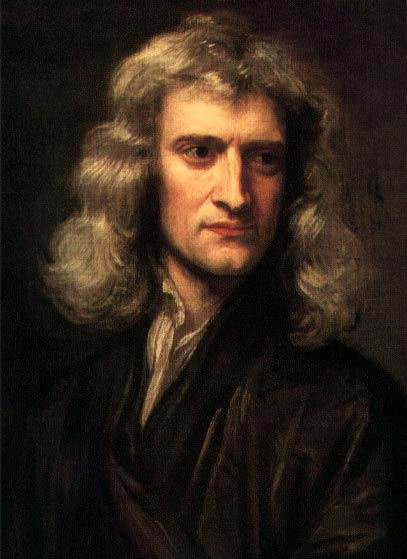
\includegraphics[scale=0.3]{newton_portrait.jpg} \\
\end{tabular}\end{center}

\subsection*{Biographie}

\subsubsection*{Jeunesse}

L'Angleterre n'ayant alors pas encore adopté le 
\htmladdnormallink{calendrier grégorien}{http://fr.wikipedia.org/wiki/Calendrier\_gr\%C3\%A9gorien},
la date de naissance d’Isaac Newton est enregistrée en date du 25 décembre 1642,
au manoir de Woolsthorpe près de Grantham, dans le Lincolnshire (Angleterre),
de parents paysans. 
À cinq ans, il fréquente l’école primaire de Skillington, puis à
douze ans celle de Grantham.

\subsubsection*{Newton à Cambridge}

À dix-huit ans, il entre alors au Trinity College de Cambridge (il y restera
sept ans), où il se fait remarquer par son maître, Isaac Barrow. Il a également
comme professeur Henry More qui l'influencera dans sa conception de l'espace
absolu.

\subsection*{Théories scientifiques}

Quant à la méthode, Newton n'accepte que les relations mathématiques découvertes
par l'observation rigoureuse des phénomènes. D'où sa fameuse formule :

	\begin{quotation}
 Je ne feins pas d'hypothèses \textit{(Hypotheses non fingo)}.
	\end{quotation}

% LaTeX2e code generated by txt2tags 2.6. (http://txt2tags.org)
% cmdline: txt2tags -t tex newton.t2t
\end{document}
